\section{Расчет биологической защиты} %TODO: убрать для репорта
\subsection{Постановка задачи}
Необходимо рассчитать дозу облучения при стационарном режиме работы ЯЭУ ВВЭР-1000 за биологической защитой

\subsection{Построение расчетной модели биологической защиты}
Для формирования расчетной модели рассмотрим компоновку элементов и помещений ЯЭУ с РУ ВВЭР-1000.

\begin{figure}[H]
	\begin{center}
		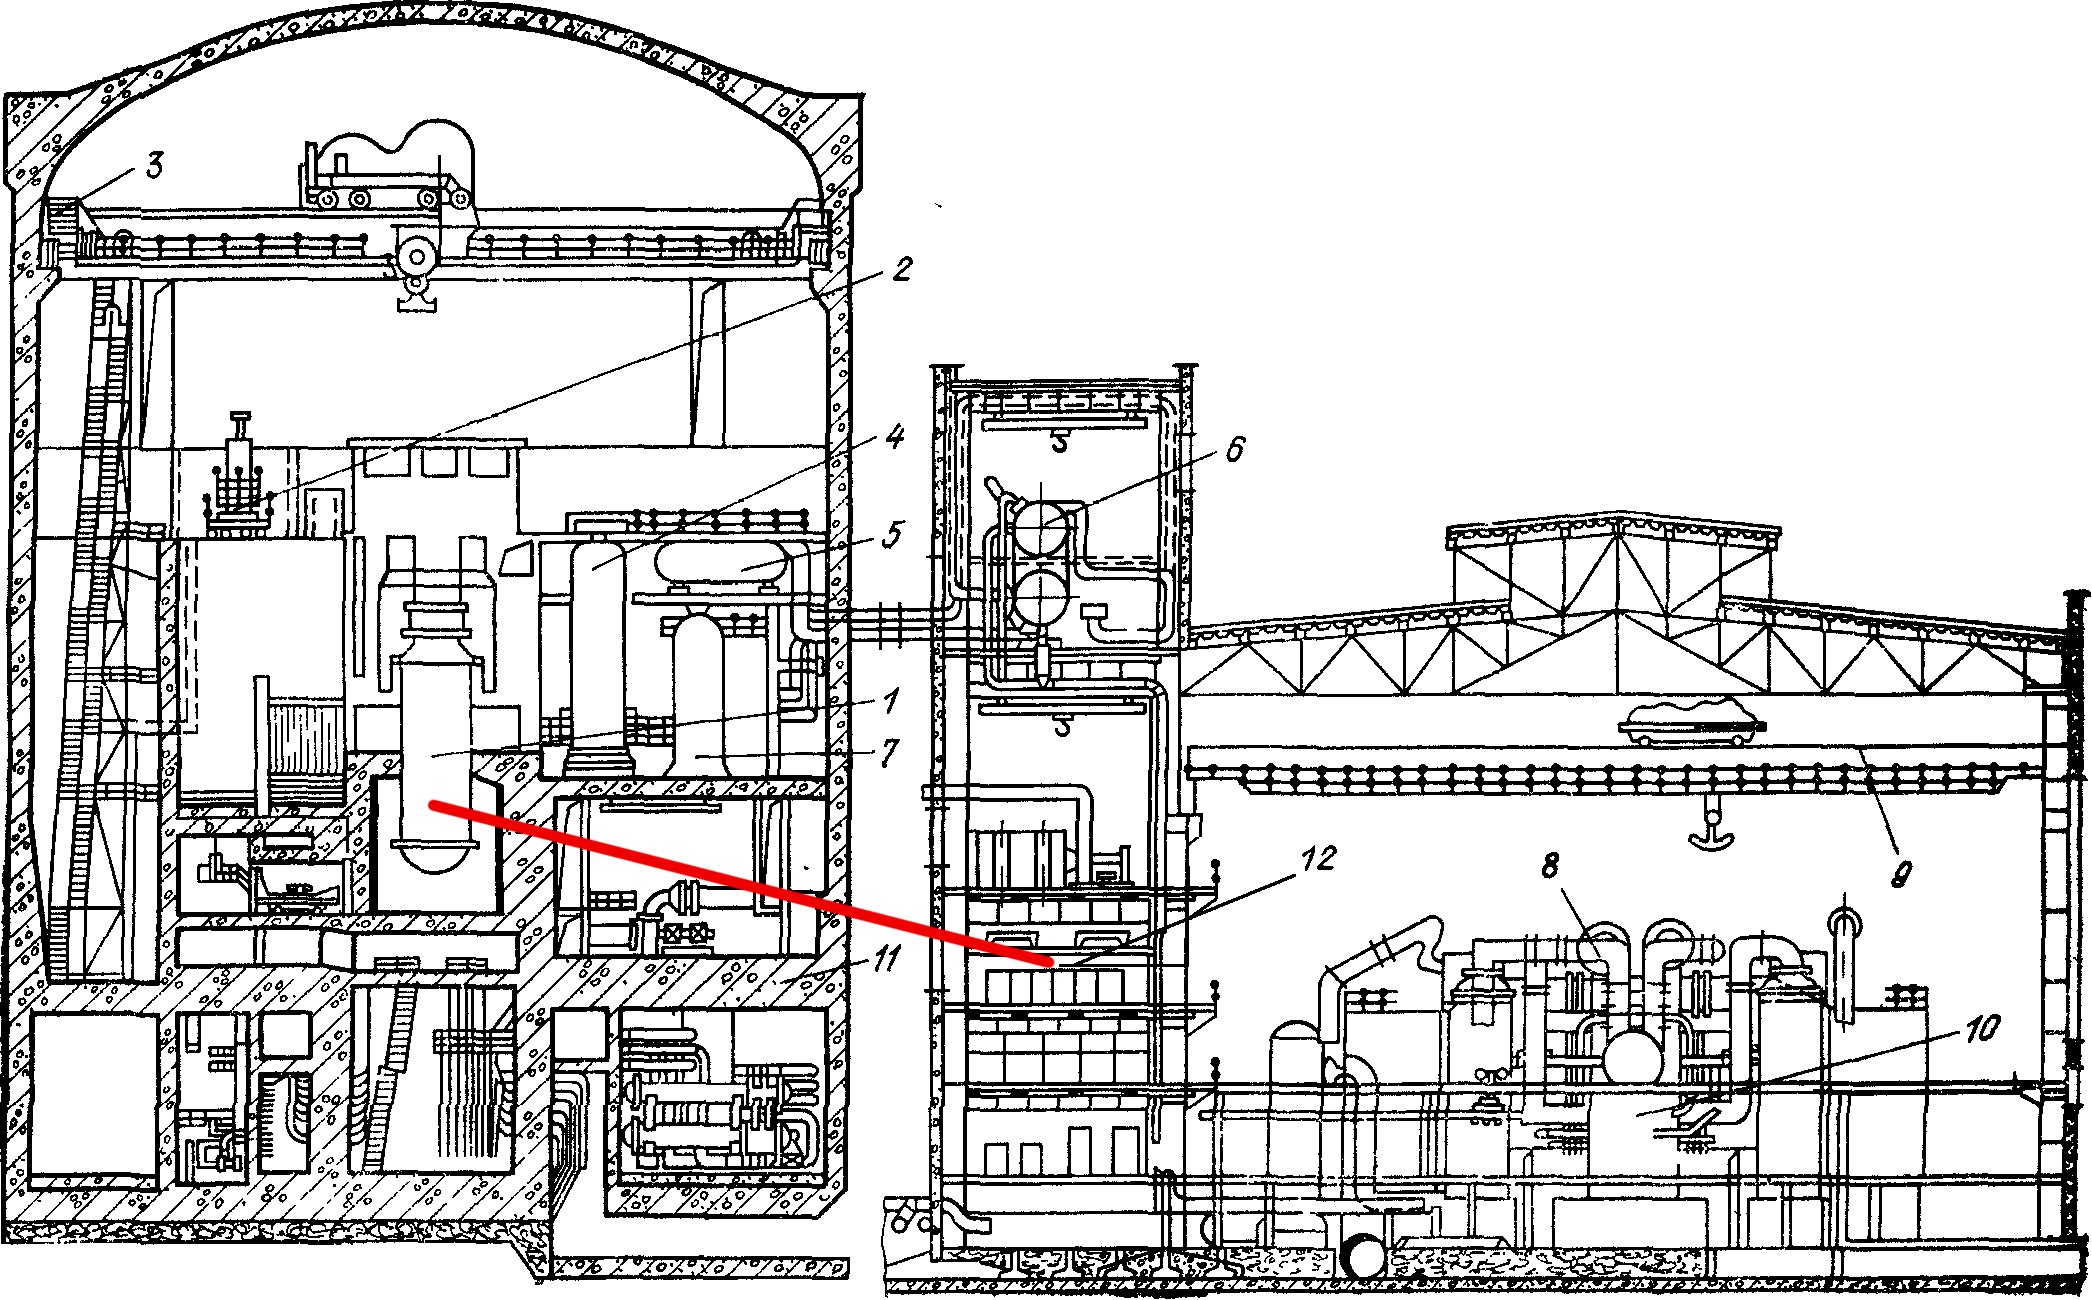
\includegraphics{razrez_bio.png}
		\caption{
			Общая компоновка энергоблока с РУ ВВЭР-1000 (Южно-Украинская АЭС): \\
			1 — реактор; 2 — машина для перегрузки топлива; 3 — подъемный кран реакторного отделения; 4 — компенсатор давления, 5 — барботер; 6 — деаэратор; 7 — гидроемкость, 8 — турбогенератор; 9 — подъемный кран машинного зала; 10 — регенеративные подогреватели, 11 —  защитная оболочка
		}
		\label{pic:razrez_bio} % название для ссылок внутри кода
	\end{center}
\end{figure}
% Монахов Атомные электрические станции и их технологическое оборудование

\paragraph{Элементы компоновки вокруг реактора}

Рассмотрим основные элементы защиты, внешние по отношению к ВВЭР-1000 в сборе. Корпус реактора установливается в \textit{бетонную шахту} [\ref{pic:beton_shakhta}], которая играет роль основной опоры и крепления реактора с учетом сейсмических нагрузкок, а также биологической защиты от излучения со стороны АЗ. Между корпусом реактора и шахтой имеется кольцевой зазор, предназначенный для периодического контроля металла корпуса в связи с требованиями правил. Шахта резделена по высоте на два объема разделительным сильфоном: 
\begin{itemize}
	\item Верхний, снабжен гидрозатвором и соединяется с бассейном выдержки. При перегрузке верхний объем шахты вместе с бассейном заливается водой.
	\item Нижний, условно разделяемый фермой опорной на шахту зоны патрубков и шахту цилиндрической части корпуса. Соединяется проемом, снабженным герметичной дверью, с помещением для машины осмотра корпуса.
\end{itemize}
В помещении зоны патрубков
биологическая защита выполнена из металлических коробов, заполненных специальным составом, в который входят серпентинитовая галя, кристаллический карбид бора, дробь чугунная литая. В районе активной зоны применяется «сухая» защита, которая представляет из себя слой серпентинитового бетона толщиной
720 мм и высотой 4,7 м, облицованного металлической оболочкой. Такой бетон обладает высокой радиационной стойкостью, что позволяет удовлетворить требования по нейтронной защите.

\begin{figure}[H]
	\begin{center}
		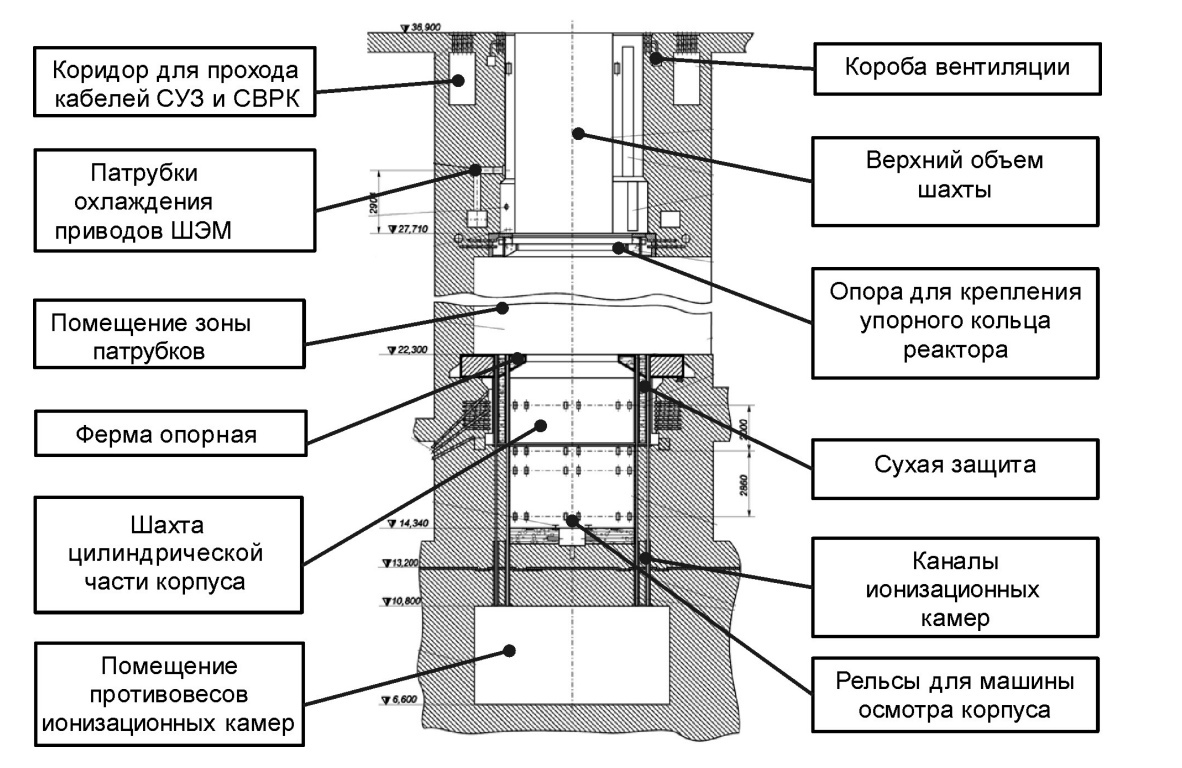
\includegraphics[scale=0.4]{beton.jpg}
		\caption{
			Бетонная шахта реактора
		}
		\label{pic:beton_shakhta} % название для ссылок внутри кода
	\end{center}
\end{figure}



Все оборудование первого контура заключено в цилиндрическую оболочку, в верхней части которой расположен грузоподъемный поворотный кран. Между реакторным и машинным залами располагается этажерка электротехнических устройств, где размещены также деаэраторы и различные лаборатории.

\paragraph{Активная зона}
\paragraph{Внутрикорпусная шахта}
\paragraph{Корпус}
\paragraph{Бетонная шахта}
\paragraph{Защитная оболочка}